\section{The Monte Carlo Method: Gambling with Integrals During Wartime}

The year is 1946. The world has just come out of World War II. Los Alamos is still echoing with the ghost of fission, and physicists are faced with a new challenge: how do you simulate complex systems—like neutron diffusion in a nuclear reactor—without solving monstrous integrals by hand?

Enter Stanislaw Ulam.

While recovering from an illness (and also while playing an actual game of solitaire), Ulam had an epiphany: what if, instead of trying to compute an integral analytically, you could just throw darts at it? Not real darts—\textit{probabilistic} ones.

\begin{quote}
\textit{“What if I could estimate the behavior of particles not by solving equations, but by simulating their random journeys?”}
\end{quote}

He brought this idea to John von Neumann, who immediately saw its potential. But this was still the 1940s—so they named it after the most glamorous, luck-driven place they could think of:

\begin{quote}
\textbf{Monte Carlo.}
\end{quote}

It was a joke. But also a revolution.

\begin{example}[title={Monte Carlo: Estimating Integrals by Playing with Chance}]
Imagine trying to compute an ugly multidimensional integral:

\[
I = \int_D f(x)\, dx
\]

But the domain \( D \) is complicated, and the function \( f(x) \) has no closed-form antiderivative. Instead of wrestling with the integral directly, the Monte Carlo method lets you approximate it using randomness:

\begin{enumerate}
  \item Sample \( N \) random points \( x_1, x_2, \ldots, x_N \) uniformly over \( D \).
  \item Evaluate the function at each point: \( f(x_1), f(x_2), \ldots, f(x_N) \).
  \item Take the average:
  \[
  \hat{I} = \frac{\text{Volume}(D)}{N} \sum_{i=1}^N f(x_i)
  \]
\end{enumerate}

This gives an estimate \( \hat{I} \) for the true value of the integral \( I \), and it converges as \( N \to \infty \), thanks to the Law of Large Numbers.

\medskip

\noindent\textbf{Conclusion:} Monte Carlo integration replaces algebra with randomness. Instead of solving equations, you run simulations—and let probability do the heavy lifting.

\begin{quote}
When brute force fails, roll the dice.
\end{quote}
\end{example}


\subsubsection{Why It Worked (Even Then)}

Monte Carlo didn’t care about symbolic forms. It worked by sampling random inputs, simulating outcomes, and averaging the results. It was:

\begin{itemize}
  \item Scalable to high dimensions (where traditional integration fails)
  \item Easy to parallelize (each random trial is independent)
  \item Amenable to early computing hardware
\end{itemize}

And it did something more profound: it let physicists \textbf{approximate integrals} without needing closed-form solutions. No more wrangling infinite series or inventing substitutions from scratch. Just simulate enough outcomes, and the law of large numbers would do the rest.

\subsubsection{From Neutrons to Neural Nets}

Monte Carlo was born in the nuclear age, but it thrives in the information age.

It’s at the heart of:

\begin{itemize}
  \item Bayesian inference
  \item Reinforcement learning
  \item Variational autoencoders
  \item Policy gradient estimation
\end{itemize}

Anywhere you need to integrate over uncertainty, but can't symbolically—Monte Carlo steps in. And today, those random samples get stuffed into matrices and processed by GPUs, bringing us full circle from wartime physics to deep learning.

\begin{quote}
Monte Carlo started as a gamble to simulate the unknowable.  
Now it’s a workhorse for approximating the intractable.
\end{quote}



\subsection{Monte Carlo as Matrix Math}

Monte Carlo methods don’t start as matrix-based—but they become matrix-friendly when scaled. Suppose we want to estimate an integral of the form:

\[
\mathbb{E}[f(X)] = \int f(x) \, p(x) \, dx
\]

We approximate this using \( N \) random samples \( x_1, x_2, \ldots, x_N \) drawn from \( p(x) \), and compute:

\[
\frac{1}{N} \sum_{i=1}^N f(x_i)
\]

Now organize the samples into a matrix:

\[
X \in \mathbb{R}^{N \times d} \quad \text{(each row is a $d$-dimensional sample)}
\]

Then evaluate the function on each row:

\[
f(X) \in \mathbb{R}^N \quad \text{(vector of function values)}
\]

Finally, multiply by a weight vector \( w \in \mathbb{R}^N \) (uniform or importance-sampled):

\[
\text{Integral estimate} = w^\top f(X)
\]

This is a dot product. A single matrix–vector multiply. Monte Carlo integration becomes linear algebra.


\subsubsection{Worked Example: Monte Carlo Integration as a Dot Product}

Let’s walk through a concrete example. Suppose we want to estimate the expected value of the function \( f(x) = \sin(x) \) under a probability distribution \( p(x) \), where \( x \sim \mathcal{U}[0, \pi] \). That is:

\[
\mathbb{E}[f(X)] = \int_0^\pi \sin(x) \cdot \frac{1}{\pi} \, dx
\]

This integral has an exact value:

\[
\int_0^\pi \frac{\sin(x)}{\pi} \, dx = \frac{2}{\pi}
\]

Let’s now approximate it using Monte Carlo sampling with \( N = 5 \) samples.

\paragraph{Step 1: Draw Samples}

We sample \( x_1, x_2, \ldots, x_5 \) uniformly from the interval \( [0, \pi] \):

\[
X = 
\begin{bmatrix}
0.3 \\
1.2 \\
2.1 \\
2.7 \\
3.0
\end{bmatrix}
\]

\paragraph{Step 2: Evaluate the Function}

Compute \( f(x_i) = \sin(x_i) \) for each row:

\[
f(X) =
\begin{bmatrix}
\sin(0.3) \\
\sin(1.2) \\
\sin(2.1) \\
\sin(2.7) \\
\sin(3.0)
\end{bmatrix}
\approx
\begin{bmatrix}
0.2955 \\
0.9320 \\
0.8632 \\
0.4274 \\
0.1411
\end{bmatrix}
\]

\paragraph{Step 3: Assign Weights}

Since the distribution is uniform over \( [0, \pi] \), each sample gets equal weight \( w_i = \frac{1}{N} \cdot \pi \), giving:

\[
w =
\begin{bmatrix}
\frac{\pi}{5} \\
\frac{\pi}{5} \\
\frac{\pi}{5} \\
\frac{\pi}{5} \\
\frac{\pi}{5}
\end{bmatrix}
\]

\paragraph{Step 4: Compute the Estimate as a Dot Product}

\[
\hat{I} = w^\top f(X) = \frac{\pi}{5} \cdot (0.2955 + 0.9320 + 0.8632 + 0.4274 + 0.1411)
\]

\[
\hat{I} \approx \frac{\pi}{5} \cdot 2.6592 \approx 0.5289
\]

The true value is \( \frac{2}{\pi} \approx 0.6366 \), so even with only 5 samples, the estimate is close—and this improves with more samples.

\paragraph{Bottom Line:}

\[
\text{Monte Carlo Integral} = w^\top f(X)
\]

What looks like numerical integration is just a weighted sum—a dot product. Monte Carlo becomes matrix math.





\subsection{Parallelism, Tensors, and GPU Firepower}

Here’s where things scale:

\begin{itemize}
  \item All \( N \) evaluations of \( f(x_i) \) can be computed in parallel.
  \item The weight application becomes a \texttt{matmul} (matrix multiplication).
  \item GPU cores apply the same operation to many data points: SIMD (Single Instruction, Multiple Data).
\end{itemize}

If we perform Monte Carlo estimates across many functions (as in Bayesian inference, variational methods, or neural net training), we can organize:

\begin{itemize}
  \item Samples as a matrix \( X \in \mathbb{R}^{N \times d} \)
  \item Function outputs as a matrix \( F \in \mathbb{R}^{N \times m} \)
  \item Weights as a vector \( w \in \mathbb{R}^{N} \)
\end{itemize}

Then compute:

\[
w^\top F \in \mathbb{R}^m
\]

This is just a weighted average across batch outputs—used everywhere in deep learning, from loss functions to layer aggregation.



\begin{figure}[H]
\centering
\begin{tikzpicture}[node distance=1.8cm and 2.5cm, auto, thick, >=stealth, scale=1, every node/.style={transform shape}]

  % Input Matrix X
  \node[draw, rectangle, minimum width=3.5cm, minimum height=1.8cm, fill=blue!10] (X) {\(\mathbf{X} \in \mathbb{R}^{N \times d}\)};
  \node[below=0.15cm of X] {\scriptsize Sample points};

  % f(X)
  \node[draw, rectangle, right=of X, minimum width=2.5cm, minimum height=1.2cm, fill=orange!20] (fX) {\(\mathbf{f}(\mathbf{X}) \in \mathbb{R}^N\)};
  \node[below=0.15cm of fX] {\scriptsize Evaluate function};

  % Weight vector
  \node[draw, rectangle, below=1.2cm of fX, minimum width=2.2cm, minimum height=1cm, fill=green!20] (w) {\(\mathbf{w} \in \mathbb{R}^N\)};
  \node[below=0.15cm of w] {\scriptsize Weights (uniform or adaptive)};

  % Dot product
  \node[draw, circle, right=of fX, minimum size=1.2cm, fill=gray!15] (dot) {\(\cdot\)};
  \node[below=0.15cm of dot] {\scriptsize Weighted sum};

  % Output estimate
  \node[draw, rectangle, right=of dot, minimum width=2.5cm, minimum height=1.2cm, fill=purple!20] (I) {\(\hat{I} \approx \mathbf{w}^\top \mathbf{f}(\mathbf{X})\)};
  \node[below=0.15cm of I] {\scriptsize Integral estimate};

  % Arrows
  \draw[->] (X) -- (fX);
  \draw[->] (fX) -- (dot);
  \draw[->] (w) -- (dot);
  \draw[->] (dot) -- (I);

\end{tikzpicture}
\caption{Matrix-based Monte Carlo integration: points \(\mathbf{X}\) are sampled and evaluated by \(\mathbf{f(X)}\), multiplied with weights \(\mathbf{w}\), and summed for an integral estimate. All steps can be parallelized.}
\label{fig:monte-carlo-matrix}
\end{figure}



\subsection{The Echo of Measure Theory}

This isn’t just engineering. It’s a reinterpretation of Lebesgue’s idea:

\begin{quote}
Integration is a weighted sum over sets. In modern ML, we approximate those sets by samples, and the weights become vectors. The integral becomes a dot product.
\end{quote}

Where Lebesgue used sets and indicator functions, we use tensors and matrix multiplications.

\subsection{From Measurable Functions to Neural Networks}

A neural network is just a function \( f_\theta(x) \) that we optimize over a dataset \( X \). During training, we compute expectations of loss:

\[
\mathbb{E}_{x \sim p(x)} [\ell(f_\theta(x), y)] \approx \frac{1}{N} \sum_{i=1}^N \ell(f_\theta(x_i), y_i)
\]

The structure of this computation mirrors the structure of Monte Carlo integration. It’s just:

\begin{itemize}
  \item Evaluate a function over a sampled set
  \item Weight the evaluations
  \item Take a sum
\end{itemize}

Which is, in essence, an integral. But done in parallel. Through layers of matrix multiplication.

\subsection{Conclusion: Linear Algebra as the Executor of Measure Theory}

In the 1940s, inside the secret labs of Los Alamos, John von Neumann and Stan Ulam weren’t thinking about generating cat pictures. They were trying to calculate the probability that a neutron, moving through a chunk of fissile material, would trigger a chain reaction. The integrals involved were so complex — involving random trajectories, particle collisions, and uncertain inputs — that classical calculus was no match. So they invented something new: the Monte Carlo method.

The idea was simple but radical. If you can’t compute an integral exactly, throw darts — sample randomly from the space, and average the results. The method was named after the Monte Carlo casino because, as Ulam joked, his uncle kept losing money there — and randomness seemed to be the family tradition.

But randomness on its own isn’t enough. To tame these probabilistic guesses and make them computationally efficient, you need structure. That’s where linear algebra enters the story. It turns distributions into vectors, expectations into matrix multiplications, and massive sampling into tractable tensor operations.

Just as Fourier analysis decomposed functions into waves, linear algebra decomposes integration into dot products. Measure theory tells us what to integrate — probability distributions, likelihood functions, expected values. Monte Carlo tells us we can sample instead of solve. And linear algebra makes it fast.

This is why modern machine learning looks the way it does:
\begin{itemize}
  \item Our datasets are matrices
  \item Our operations are vectorized
  \item Our integrals are replaced with sums
  \item And our sums are accelerated by GPUs
\end{itemize}

Today, the same technique used to estimate neutron diffusion in hydrogen bombs is used to train neural networks and generate photorealistic images. The randomness hasn’t changed — only the stakes.

\begin{quote}
Lebesgue taught us what to integrate.  
Von Neumann showed us how to sample it.  
Linear algebra taught us how to do it fast.
\end{quote}


\subsection{Von Neumann Architecture: The Blueprint of Classical Computing}

The Von Neumann architecture laid the groundwork for nearly every traditional computer. Its key features include:

\begin{itemize}
    \item \textbf{Unified Memory}: Both program instructions and data reside in the same memory.
    \item \textbf{Central Processing Unit (CPU)}: Contains an Arithmetic Logic Unit (ALU) and a Control Unit.
    \item \textbf{Sequential Execution}: The CPU fetches, decodes, and executes instructions in order.
    \item \textbf{Single Bus}: A shared pathway handles both instructions and data, limiting parallelism.
\end{itemize}

In simple terms, it’s like a kitchen where the chef must retrieve both the recipe and ingredients from the same drawer, one step at a time.

\section*{The MANIAC Machine: A Von Neumann Computer in the Atomic Age}

Built in the early 1950s at Los Alamos by Nicholas Metropolis, the MANIAC I (\textit{Mathematical Analyzer, Numerical Integrator, and Computer}) faithfully implemented the Von Neumann model.

\begin{tcolorbox}[title=Quick Spec Summary,fonttitle=\bfseries, colback=gray!10]
\begin{itemize}
    \item \textbf{Memory:} Electrostatic tubes and magnetic drum storage
    \item \textbf{Word Size:} 40 bits
    \item \textbf{Execution:} Serial processing (one bit at a time)
    \item \textbf{Programming:} Machine language, no OS
    \item \textbf{Applications:} Monte Carlo simulations, thermonuclear computations, chess playing
\end{itemize}
\end{tcolorbox}

\subsection{How MANIAC Mapped to Von Neumann Architecture}

\begin{table}[h!]
\centering
\begin{tabular}{@{}ll@{}}
\toprule
\textbf{Von Neumann Component} & \textbf{MANIAC Implementation} \\ \midrule
Memory & Electrostatic + magnetic drum storage \\
Control Unit & Hardwired logic for sequential instruction decoding \\
ALU & Performed basic arithmetic and logic operations \\
Program \& Data Storage & Shared memory space (stored-program concept) \\
Execution Cycle & Fetch $\rightarrow$ Decode $\rightarrow$ Execute $\rightarrow$ Repeat \\ \bottomrule
\end{tabular}
\caption{Mapping the Von Neumann model onto the MANIAC machine}
\end{table}

\section{Why It Mattered}

The MANIAC wasn’t just a theoretical exercise—it was a practical tool. It brought Von Neumann’s ideas to life and helped solve cutting-edge problems in physics and cryptography. From simulating nuclear reactions to exploring the frontiers of computation, it showed what a computer could be.

\medskip


\begin{figure}[H]
  \centering
  \begin{tikzpicture}[
    block/.style={rectangle, draw, minimum width=3.5cm, minimum height=1.2cm, align=center},
    subblock/.style={rectangle, draw, minimum width=2.5cm, minimum height=1cm, align=center},
    arrow/.style={-{Latex}, thick}
  ]
  
  % Memory
  \node[block, fill=gray!10] (memory) {Main Memory\\(Program + Data)};
  
  % CPU box
  \node[block, right=5cm of memory, fill=gray!10] (cpu) {CPU};
  
  % ALU and Control inside CPU
  \node[subblock, above=0.1cm of cpu.center, yshift=0.6cm] (alu) {Arithmetic Logic Unit (ALU)};
  \node[subblock, below=0.1cm of cpu.center, yshift=-0.6cm] (cu) {Control Unit};
  
  % I/O
  \node[block, below=3cm of memory, fill=gray!10] (io) {Input / Output};
  
  % Bus arrows
  \draw[arrow] (memory) -- (cpu) node[midway, above, sloped] {Data / Instructions};
  \draw[arrow] (cpu) -- (memory) node[midway, below, sloped] {Store / Load};
  
  \draw[arrow] (cpu) -- (io) node[midway, right] {Output};
  \draw[arrow] (io) -- (cpu) node[midway, left] {Input};
  
  % Dashed box for CPU internals
  \begin{scope}[on background layer]
    \node[draw, dashed, fit=(alu)(cu), inner sep=6pt, label=right:{\small Von Neumann CPU}] {};
  \end{scope}
  \end{tikzpicture}
    
  \caption{Von Neumann Architecture: Core Components Used in the MANIAC Machine}
  \end{figure}


  \medskip



  \begin{figure}[H]
    \centering
    \begin{tikzpicture}[
      block/.style={rectangle, draw, minimum width=3.5cm, minimum height=1.2cm, align=center, fill=gray!10},
      subblock/.style={rectangle, draw, minimum width=2.5cm, minimum height=1cm, align=center},
      clockblock/.style={rectangle, draw, minimum width=2.5cm, minimum height=1cm, align=center, fill=yellow!20},
      arrow/.style={-{Latex}, thick}
    ]
    
    % Memory
    \node[block] (memory) {Main Memory\\(Program + Data)};
    
    % CPU box
    \node[block, right=5cm of memory] (cpu) {CPU};
    
    % ALU and Control inside CPU
    \node[subblock, above=0.1cm of cpu.center, yshift=0.6cm] (alu) {Arithmetic Logic Unit (ALU)};
    \node[subblock, below=0.1cm of cpu.center, yshift=-0.6cm] (cu) {Control Unit};
    
    % Clock Control
    \node[clockblock, above=2.2cm of cpu] (clock) {Clock / Timing Control};
    
    % I/O
    \node[block, below=3cm of memory] (io) {Input / Output};
    
    % Bus arrows
    \draw[arrow] (memory) -- (cpu) node[midway, above, sloped] {Data / Instructions};
    \draw[arrow] (cpu) -- (memory) node[midway, below, sloped] {Store / Load};
    
    \draw[arrow] (cpu) -- (io) node[midway, right] {Output};
    \draw[arrow] (io) -- (cpu) node[midway, left] {Input};
    
    % Clock arrows
    \draw[arrow] (clock) -- (cpu.north) node[midway, right=2pt] {\footnotesize Sync};
    \draw[arrow] (clock) -- (memory.north) node[midway, left=2pt] {\footnotesize Control Signal};
    
    % Dashed box for CPU internals
    \begin{scope}[on background layer]
      \node[draw, dashed, fit=(alu)(cu), inner sep=6pt, label=right:{\small Von Neumann CPU}] {};
    \end{scope}
    
    \end{tikzpicture}

    \caption{Von Neumann Architecture with Clock / Timing Control (as in the MANIAC Machine)}
  \end{figure}

  \medskip
  
  \begin{tcolorbox}[colback=gray!5!white,colframe=black!75!white,title=Historical Sidebar: Nicholas Metropolis and the Monte Carlo Method,fonttitle=\bfseries]

    In the 1940s, while most people were calculating tips at diners, Nicholas Metropolis and his colleagues were calculating atomic bomb behavior. Working at Los Alamos, Metropolis faced a problem: how do you model incredibly complex physical systems—like nuclear reactions—when the equations are too gnarly to solve directly?
    
    Their answer? \textbf{Guess. A lot. And keep the good guesses.}
    
    Inspired by statistical physics and the randomness of casino games, Metropolis and his team developed what became known as the \textbf{Monte Carlo method}. The idea was simple but revolutionary: use random sampling to explore possible states of a system, weighting the outcomes by probability. The code name was a nod to the Monte Carlo Casino in Monaco—legend has it that Stanislaw Ulam had an uncle who gambled there.
    
    The Monte Carlo method would go on to power everything from neutron diffusion models to weather forecasts to deep learning. But in the beginning, it was about nuclear physics, roulette wheels, and the birth of probabilistic computing.
    
    And yes, Metropolis also lent his name to the \textit{Metropolis algorithm}, the ancestor of modern MCMC techniques—because when you invent how computers guess, you get naming rights.
    
    \end{tcolorbox}



    \section{What the MANIAC Monte Carlo Did (in Brief)}

    Let's say we want to estimate \( \pi \) using a simple Monte Carlo method—throw darts at a unit square and count how many fall inside the unit circle. The basic idea is to randomly generate points \((x, y)\) such that \(0 \leq x, y \leq 1\), and then determine whether they fall inside the unit circle by checking:
    
    \[
    x^2 + y^2 \leq 1
    \]
    
    If they do, they're counted as a "hit." The estimate for \( \pi \) is then given by:
    
    \[
    \pi \approx 4 \cdot \frac{\text{Number of points inside circle}}{\text{Total number of points}}
    \]
    
    This method works because the ratio of the area of the unit circle quadrant to the unit square is \( \pi/4 \).
    
    \subsection{MANIAC Style Instruction Format (Simplified)}
    
    The MANIAC used 40-bit words, and each instruction looked something like this:
    
    \begin{itemize}
        \item \textbf{Opcode} — the operation code, e.g. \texttt{01 = Add}, \texttt{02 = Subtract}, \texttt{03 = Load}, etc.
        \item \textbf{Memory Address} — where the operand lives
        \item \textbf{Modifier} (optional) — for things like indirect addressing
    \end{itemize}
    
    Each line was usually entered as a raw number, not as text—but in this document, we'll use readable mnemonics for clarity.
    


    \begin{figure}[H]
      \centering
      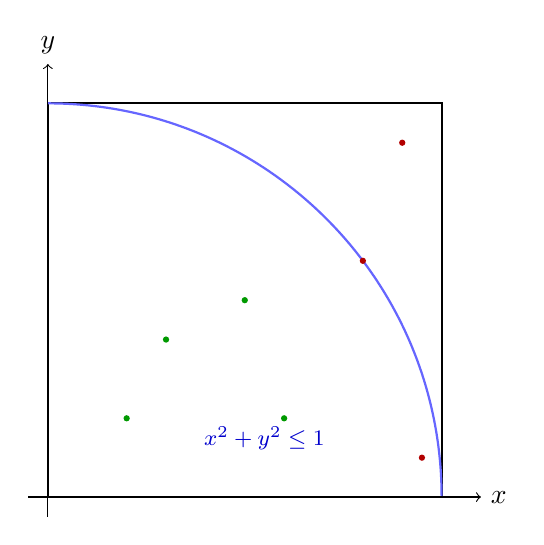
\begin{tikzpicture}[scale=5]
      
      % Draw the unit square
      \draw[thick] (0,0) rectangle (1,1);
      
      % Draw the quarter circle inside the square (from (1,0) to (0,1))
      \draw[thick, blue!60] (1,0) arc[start angle=0, end angle=90, radius=1];
      
      % Label axes
      \draw[->] (-0.05,0) -- (1.1,0) node[right] {$x$};
      \draw[->] (0,-0.05) -- (0,1.1) node[above] {$y$};
      
      % Draw some example darts
      \fill[green!60!black] (0.3,0.4) circle(0.008); % hit
      \fill[green!60!black] (0.6,0.2) circle(0.008); % hit
      \fill[red!70!black] (0.8,0.6) circle(0.008); % miss
      \fill[green!60!black] (0.5,0.5) circle(0.008); % hit
      \fill[red!70!black] (0.9,0.9) circle(0.008); % miss
      \fill[green!60!black] (0.2,0.2) circle(0.008); % hit
      \fill[red!70!black] (0.95,0.1) circle(0.008); % miss
      
      % Label quarter circle
      \node at (0.55,0.15) [blue!80!black] {\footnotesize $x^2 + y^2 \leq 1$};
      
      \end{tikzpicture}
      \caption{Monte Carlo Simulation: Darts Inside a Unit Square and Quarter Circle}
      \label{fig:montecarlo_quartercircle}
      \end{figure}


      \tikzset{
        block/.style={rectangle, draw, minimum width=3.5cm, minimum height=1.1cm, text centered, fill=blue!10},
        decision/.style={diamond, draw, minimum width=3.5cm, minimum height=1.2cm, text centered, aspect=2, fill=yellow!20},
        io/.style={trapezium, trapezium left angle=70, trapezium right angle=110, draw, fill=green!20, text centered},
        arrow/.style={thick, -{Latex[]}},
      }
     
      \medskip

      \begin{figure}[H]
      \centering
      \begin{tikzpicture}[node distance=1.7cm]
      
      \node[block] (start) {START};
      \node[block, below of=start] (genx) {Generate Random X};
      \node[block, below of=genx] (geny) {Generate Random Y};
      \node[block, below of=geny] (xsq) {XSQ = X × X};
      \node[block, below of=xsq] (ysq) {YSQ = Y × Y};
      \node[block, below of=ysq] (r2) {RADIUS² = XSQ + YSQ};
      \node[decision, below of=r2, yshift=-0.2cm] (checkhit) {$x^2 + y^2 < 1?$};
      
      \node[block, right=3.5cm of checkhit] (incrhit) {Increment HIT\_COUNT};
      \node[block, below of=checkhit, yshift=-1.3cm] (incrtrial) {Increment TRIAL\_COUNT};
      \node[decision, below of=incrtrial, yshift=-0.3cm] (checkdone) {TRIAL\_COUNT $\ge$ MAX\_TRIALS?};
      
      \node[block, right=3.5cm of checkdone] (piest) {Estimate $\pi = 4 \cdot \frac{\text{HIT\_COUNT}}{\text{TRIAL\_COUNT}}$};
      \node[block, below of=checkdone, yshift=-1.3cm] (loop) {Repeat Loop};
      
      % Arrows
      \draw[arrow] (start) -- (genx);
      \draw[arrow] (genx) -- (geny);
      \draw[arrow] (geny) -- (xsq);
      \draw[arrow] (xsq) -- (ysq);
      \draw[arrow] (ysq) -- (r2);
      \draw[arrow] (r2) -- (checkhit);
      
      \draw[arrow] (checkhit) -- node[above] {yes} (incrhit);
      \draw[arrow] (checkhit) -- node[left] {no} (incrtrial);
      \draw[arrow] (incrhit) |- (incrtrial);
      
      \draw[arrow] (incrtrial) -- (checkdone);
      \draw[arrow] (checkdone) -- node[above] {yes} (piest);
      \draw[arrow] (checkdone) -- node[left] {no} (loop);
      \draw[arrow] (loop.west) -- ++(-3.5,0) |- (genx.west);
      
      \end{tikzpicture}
      \caption{Flowchart for Monte Carlo Simulation to Estimate $\pi$}
      \label{fig:montecarlo_flowchart}
    \end{figure}
      
      


\begin{tcolorbox}[title=Monte Carlo Simulation for \(\pi\), colback=gray!5, colframe=black]
  \ttfamily
  
  ; Monte Carlo to estimate $\pi$ using MANIAC-style pseudocode\par
  
  START:\par
  \quad LOAD RND\_SEED\_X         ; Load initial seed\par
  \quad CALL RANDOM\_GEN         ; Generate random X between 0 and 1\par
  \quad STORE X\par
  
  \quad LOAD RND\_SEED\_Y         ; Load another seed\par
  \quad CALL RANDOM\_GEN         ; Generate random Y between 0 and 1\par
  \quad STORE Y\par
  
  \quad LOAD X\par
  \quad MUL X\par
  \quad STORE XSQ               ; XSQ = X * X\par
  
  \quad LOAD Y\par
  \quad MUL Y\par
  \quad STORE YSQ               ; YSQ = Y * Y\par
  
  \quad LOAD XSQ\par
  \quad ADD YSQ\par
  \quad STORE RADIUS2           ; radius\^{}2 = x\^{}2 + y\^{}2\par
  
  \quad LOAD RADIUS2\par
  \quad SUB ONE                 ; Compare with 1\par
  \quad JUMPNEG INCREMENT\_HIT   ; If x\^{}2 + y\^{}2 < 1, it's a hit\par
  
  \end{tcolorbox}

      
  \begin{tcolorbox}[title=Monte Carlo Simulation for \(\pi\), colback=gray!5, colframe=black]
      \ttfamily
      
      
      NEXT\_TRIAL:\par
      \quad LOAD TRIAL\_COUNT\par
      \quad ADD ONE\par
      \quad STORE TRIAL\_COUNT\par
      \quad JUMP CHECK\_DONE\par
      
\end{tcolorbox}

\begin{tcolorbox}[title=Monte Carlo Simulation for \(\pi\), colback=gray!5, colframe=black]
  \ttfamily
  
  INCREMENT\_HIT:\par
  \quad LOAD HIT\_COUNT\par
  \quad ADD ONE\par
  \quad STORE HIT\_COUNT\par
  \quad JUMP NEXT\_TRIAL\par
  
  
\end{tcolorbox}

\begin{tcolorbox}[title=Monte Carlo Simulation for \(\pi\), colback=gray!5, colframe=black]
  \ttfamily
  
  CHECK\_DONE:\par
  \quad LOAD TRIAL\_COUNT\par
  \quad SUB MAX\_TRIALS\par
  \quad JUMPPOS COMPUTE\_PI\par
  \quad JUMP START\par
  
\end{tcolorbox}

\begin{tcolorbox}[title=Monte Carlo Simulation for \(\pi\), colback=gray!5, colframe=black]
  \ttfamily
  
  
  COMPUTE\_PI:\par
  \quad LOAD HIT\_COUNT\par
  \quad DIV TRIAL\_COUNT\par
  \quad MUL FOUR\par
  \quad STORE ESTIMATE\_PI\par
  \quad HALT\par
  
\end{tcolorbox}


\begin{tcolorbox}[title=Monte Carlo Simulation for \(\pi\), colback=gray!5, colframe=black]
  \ttfamily
  
  
  ; Constants and storage\par
  ONE:           1\par
  FOUR:          4\par
  MAX\_TRIALS:    1000\par
  X:             0\par
  Y:             0\par
  XSQ:           0\par
  YSQ:           0\par
  RADIUS2:       0\par
  HIT\_COUNT:     0\par
  TRIAL\_COUNT:   0\par
  ESTIMATE\_PI:   0\par
  RND\_SEED\_X:    1234\par
  RND\_SEED\_Y:    5678\par
  
\end{tcolorbox}


\medskip


% === Step 1 ===
\begin{figure}[H]
  \centering
  \begin{tikzpicture}[every node/.style={font=\small}, node distance=0.6cm, scale=1, transform shape]
    \node[draw, rectangle, minimum width=2.4cm, minimum height=0.8cm, fill=green!20] (input) {Input};
    \node[draw, rectangle, below=of input, minimum width=2.4cm, minimum height=0.8cm, fill=blue!10] (memory) {Memory};
    \node[draw, rectangle, right=2.5cm of memory, minimum width=3.4cm, minimum height=1.4cm] (cpu) {CPU};
    \node[draw, rectangle, below=of memory, minimum width=2.4cm, minimum height=0.8cm] (clock) {Clock};
    \draw[->, thick] (input) -- (memory) node[midway, left] {Seed X};
    \draw[->, thick, red] (memory) -- (cpu) node[midway, above] {Load RND\_SEED\_X};
    \draw[->, thick] (clock) -- (cpu);
    \draw[->, thick] (cpu) -- (memory) node[midway, below] {Store X};
  \end{tikzpicture}
  \caption{Step 1: Generate Random X}
  \end{figure}
  
  % === Step 2 ===
  \begin{figure}[H]
  \centering
  \begin{tikzpicture}[every node/.style={font=\small}, node distance=0.6cm, scale=1, transform shape]
    \node[draw, rectangle, minimum width=2.4cm, minimum height=0.8cm, fill=green!20] (input) {Input};
    \node[draw, rectangle, below=of input, minimum width=2.4cm, minimum height=0.8cm, fill=blue!10] (memory) {Memory};
    \node[draw, rectangle, right=2.5cm of memory, minimum width=3.4cm, minimum height=1.4cm] (cpu) {CPU};
    \node[draw, rectangle, below=of memory, minimum width=2.4cm, minimum height=0.8cm] (clock) {Clock};
    \draw[->, thick] (input) -- (memory) node[midway, left] {Seed Y};
    \draw[->, thick, red] (memory) -- (cpu) node[midway, above] {Load RND\_SEED\_Y};
    \draw[->, thick] (clock) -- (cpu);
    \draw[->, thick] (cpu) -- (memory) node[midway, below] {Store Y};
  \end{tikzpicture}
  \caption{Step 2: Generate Random Y}
  \end{figure}
  
  % === Step 3 ===
  \begin{figure}[H]
  \centering
  \begin{tikzpicture}[every node/.style={font=\small}, node distance=0.6cm, scale=1, transform shape]
    \node[draw, rectangle, minimum width=2.4cm, minimum height=0.8cm, fill=blue!10] (memory) {Memory};
    \node[draw, rectangle, right=2.5cm of memory, minimum width=3.4cm, minimum height=1.4cm] (cpu) {CPU (ALU)};
    \node[draw, rectangle, below=of memory, minimum width=2.4cm, minimum height=0.8cm] (clock) {Clock};
    \draw[->, thick, red] (memory) -- (cpu) node[midway, above] {Load X, MUL X};
    \draw[->, thick, red, dashed] (memory) -- ++(0,0.8) node[above] {Load Y, MUL Y};
    \draw[->, thick] (clock) -- (cpu);
    \draw[->, thick] (cpu) -- (memory) node[midway, below] {Store XSQ, YSQ};
  \end{tikzpicture}
  \caption{Step 3: Compute XSQ and YSQ}
  \end{figure}
  
  % === Step 4 ===
  \begin{figure}[H]
  \centering
  \begin{tikzpicture}[every node/.style={font=\small}, node distance=0.6cm, scale=1, transform shape]
    \node[draw, rectangle, minimum width=2.4cm, minimum height=0.8cm, fill=blue!10] (memory) {Memory};
    \node[draw, rectangle, right=2.5cm of memory, minimum width=3.4cm, minimum height=1.4cm] (cpu) {CPU (ALU)};
    \node[draw, rectangle, below=of memory, minimum width=2.4cm, minimum height=0.8cm] (clock) {Clock};
    \draw[->, thick, red] (memory) -- (cpu) node[midway, above] {XSQ + YSQ};
    \draw[->, thick] (clock) -- (cpu);
    \draw[->, thick] (cpu) -- (memory) node[midway, below] {Store RADIUS2};
  \end{tikzpicture}
  \caption{Step 4: Sum Radius Squared}
  \end{figure}
  
  % === Step 5 ===
  \begin{figure}[H]
  \centering
  \begin{tikzpicture}[every node/.style={font=\small}, node distance=0.6cm, scale=1, transform shape]
    \node[draw, rectangle, minimum width=2.4cm, minimum height=0.8cm, fill=blue!10] (memory) {Memory};
    \node[draw, diamond, right=2.5cm of memory, aspect=2, minimum height=1.4cm, draw, fill=yellow!30] (decision) {RADIUS2 < 1?};
    \node[draw, rectangle, below=of memory, minimum width=2.4cm, minimum height=0.8cm] (clock) {Clock};
    \draw[->, thick, red] (memory) -- (decision);
    \draw[->, thick] (clock) -- (decision);
  \end{tikzpicture}
  \caption{Step 5: Compare Radius to 1}
  \end{figure}
  
  % === Step 6 ===
  \begin{figure}[H]
  \centering
  \begin{tikzpicture}[every node/.style={font=\small}, node distance=0.6cm, scale=1, transform shape]
    \node[draw, rectangle, minimum width=2.4cm, minimum height=0.8cm, fill=blue!10] (memory) {Memory};
    \node[draw, rectangle, right=2.5cm of memory, minimum width=3.4cm, minimum height=1.4cm] (cpu) {CPU (ALU)};
    \node[draw, rectangle, below=of memory, minimum width=2.4cm, minimum height=0.8cm] (clock) {Clock};
    \draw[->, thick, red] (memory) -- (cpu) node[midway, above] {DIV, MUL};
    \draw[->, thick] (clock) -- (cpu);
    \draw[->, thick] (cpu) -- (memory) node[midway, below] {Store ESTIMATE\_PI};
  \end{tikzpicture}
  \caption{Step 6: Final Estimation of \(\pi\)}
  \end{figure}

\medskip


% === Step A: START ===
\begin{figure}[H]
  \centering
  \begin{tikzpicture}[every node/.style={font=\small}, node distance=0.6cm, scale=1, transform shape]
    \node[draw, ellipse, minimum width=2.5cm, minimum height=1cm, fill=gray!20] (start) {START};
    \node[draw, rectangle, below=of start, minimum width=3.5cm, minimum height=1cm] (genx) {Generate Random X};
    \node[draw, rectangle, below=of genx, minimum width=3.5cm, minimum height=1cm] (geny) {Generate Random Y};
    \draw[->, thick] (start) -- (genx);
    \draw[->, thick] (genx) -- (geny);
  \end{tikzpicture}
  \caption{START: Begin simulation and generate X and Y coordinates}
  \end{figure}
  
  % === Step B: NEXT_TRIAL ===
  \begin{figure}[H]
  \centering
  \begin{tikzpicture}[every node/.style={font=\small}, node distance=0.6cm, scale=1, transform shape]
    \node[draw, rectangle, minimum width=3.5cm, minimum height=1cm] (load) {Load TRIAL\_COUNT};
    \node[draw, rectangle, below=of load, minimum width=3.5cm, minimum height=1cm] (add) {Add 1};
    \node[draw, rectangle, below=of add, minimum width=3.5cm, minimum height=1cm] (store) {Store TRIAL\_COUNT};
    \draw[->, thick] (load) -- (add);
    \draw[->, thick] (add) -- (store);
  \end{tikzpicture}
  \caption{NEXT\_TRIAL: Increment total trial count}
  \end{figure}
  
  % === Step C: INCREMENT_HIT ===
  \begin{figure}[H]
  \centering
  \begin{tikzpicture}[every node/.style={font=\small}, node distance=0.6cm, scale=1, transform shape]
    \node[draw, rectangle, minimum width=3.5cm, minimum height=1cm] (load) {Load HIT\_COUNT};
    \node[draw, rectangle, below=of load, minimum width=3.5cm, minimum height=1cm] (add) {Add 1};
    \node[draw, rectangle, below=of add, minimum width=3.5cm, minimum height=1cm] (store) {Store HIT\_COUNT};
    \draw[->, thick] (load) -- (add);
    \draw[->, thick] (add) -- (store);
  \end{tikzpicture}
  \caption{INCREMENT\_HIT: Count a successful dart inside the circle}
  \end{figure}
  
  % === Step D: CHECK_DONE ===
  \begin{figure}[H]
  \centering
  \begin{tikzpicture}[every node/.style={font=\small}, node distance=0.6cm, scale=1, transform shape]
    \node[draw, rectangle, minimum width=3.5cm, minimum height=1cm] (load) {Load TRIAL\_COUNT};
    \node[draw, rectangle, below=of load, minimum width=3.5cm, minimum height=1cm] (sub) {Subtract MAX\_TRIALS};
    \node[draw, diamond, below=of sub, aspect=2, draw, fill=yellow!20, minimum height=1.3cm] (check) {Done?};
    \draw[->, thick] (load) -- (sub);
    \draw[->, thick] (sub) -- (check);
  \end{tikzpicture}
  \caption{CHECK\_DONE: Determine whether the simulation is complete}
  \end{figure}
  
  % === Step E: COMPUTE_PI ===
  \begin{figure}[H]
  \centering
  \begin{tikzpicture}[every node/.style={font=\small}, node distance=0.6cm, scale=1, transform shape]
    \node[draw, rectangle, minimum width=3.5cm, minimum height=1cm] (load) {Load HIT\_COUNT};
    \node[draw, rectangle, below=of load, minimum width=3.5cm, minimum height=1cm] (div) {Divide by TRIAL\_COUNT};
    \node[draw, rectangle, below=of div, minimum width=3.5cm, minimum height=1cm] (mul) {Multiply by 4};
    \node[draw, rectangle, below=of mul, minimum width=3.5cm, minimum height=1cm] (store) {Store ESTIMATE\_PI};
    \draw[->, thick] (load) -- (div);
    \draw[->, thick] (div) -- (mul);
    \draw[->, thick] (mul) -- (store);
  \end{tikzpicture}
  \caption{COMPUTE\_PI: Final estimate calculation and store result}
  \end{figure}